\section{AI Processing Pipeline}
\label{sec:ai_processing_pipeline}

The AI processing pipeline is responsible for converting a raw, multi-modal WhatsApp payload into a validated JSON record containing a task name, an ISO-8601 deadline, and a priority score. Rather than employing a dedicated NER model—which would require domain-specific training data and would fail to generalize across the linguistic diversity of group chats—the pipeline uses an instruction-tuned LLM operating under a strictly typed output schema (illustrated in Fig.~\ref{fig:ai_flow}).

\begin{figure}[tbp]
    \centering
    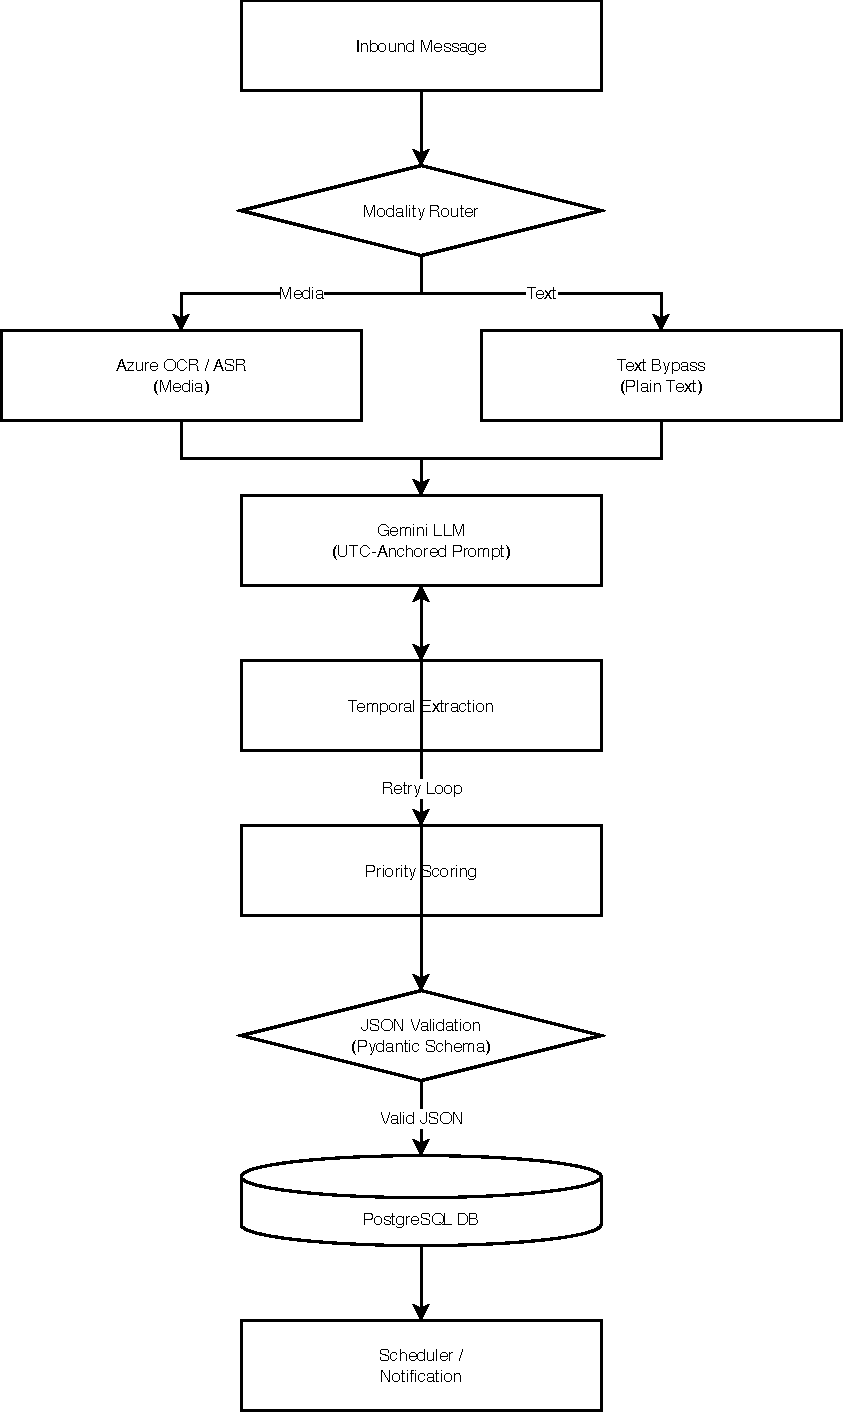
\includegraphics[width=0.95\columnwidth,keepaspectratio]{figures/Fig2_AI_Processing_Pipeline.pdf}
    \setlength{\abovecaptionskip}{4pt}
    \setlength{\belowcaptionskip}{-4pt}
    \caption{Block diagram of the AI processing pipeline. Non-text payloads are initially normalized through Azure Cognitive Services (OCR for images, ASR for audio) before the resulting UTF-8 text is passed to the Google Gemini inference layer with a UTC timestamp anchor.}
    \label{fig:ai_flow}
\end{figure}

\subsection{Multi-Modal Normalization via Azure Cognitive Services}
LLMs operate on text. Before any inference can occur, non-text content must be converted to a textual representation that preserves its semantic content. Images of whiteboards or printed schedules are processed by Azure's OCR service, which returns structured text from the image. Voice notes in \texttt{.ogg} format are routed to Azure's ASR service, producing a transcript. Both outputs are then merged with any accompanying text into a single UTF-8 string that is passed to the LLM. This design choice—using a cloud OCR/ASR service rather than on-device processing—reflects a deliberate trade-off: accuracy at the cost of network latency, which is acceptable here because non-text processing occurs asynchronously and does not block the ingestion pipeline.
